\documentclass[tikz,border=3.14mm]{standalone}
\usetikzlibrary{positioning}



\begin{document}
	\newcommand{\blok}[4]{%
		\def\sft{2pt} % shift from border of cells to coloured rectangles
		\draw[rounded corners=2pt,opacity=0.8,#1,fill=#1!50,thick] ([shift={(\sft,-\sft)}]#2.north west) rectangle ([shift={(-\sft,\sft)}]#3.south east);
		\node[right] at ([xshift=-0.44*\s cm]#2.center) {#4};}
	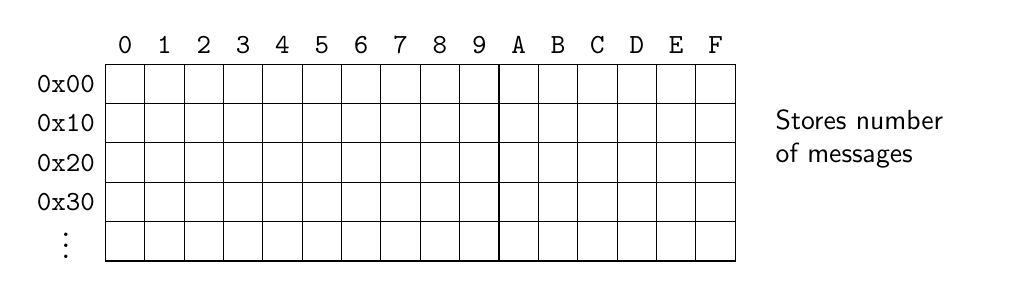
\begin{tikzpicture}[font=\ttfamily]
		
		\def\s{0.5} % size of cells
		\foreach \l [count=\k from 0] in {a,...,e}
		\foreach \i in {0,...,15}  
		\node[draw,minimum size=\s cm] (\l\i) at (\i*\s,-\k*\s){};
		\foreach \c [count=\i from 0] in {0,...,9,A,B,...,F} \node[above] at (a\i.north) {\c};
		\foreach \l [count=\i from 0] in {a,...,d} \node[left] (\l) at (\l0.west) {0x\i 0};
		\node [below= -5pt of d] {\vdots};
		
		\blok{orange}{a0}{a0}{*}
		\blok{red}{a1}{a12}{Message 1}
		\blok{olive}{a13}{a15}{M2}
		
		\blok{olive}{b0}{b7}{Message 2}
		\blok{teal}{b8}{b15}{Message 3}
		
		\blok{teal}{c0}{c15}{Message 3}
		\blok{teal}{d0}{d2}{M3}
		\blok{purple}{d3}{d9}{Message 4}
		
		\node[right,inner ysep=0 pt,minimum size=\s cm](star1) at (16*\s,0){};
		\node[minimum height=\s cm,right= 2cm  of star1](star2){};
		\blok{orange}{star1}{star2}{* Config Byte}
		\path (star1) -- (star2) node[midway,below=6pt,font=\sffamily,text width=2.5cm]{Stores number of messages};
	\end{tikzpicture}

	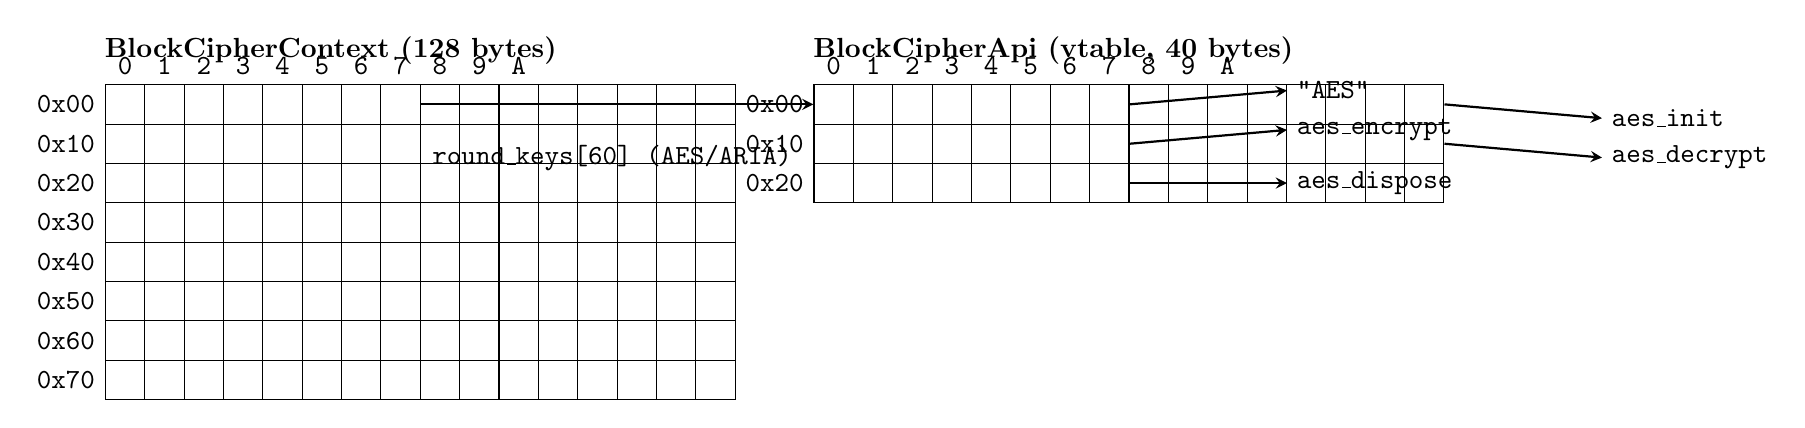
\begin{tikzpicture}[font=\ttfamily]
		\def\s{0.5} % cell size in cm
		
		%--- BlockCipherContext memory grid (8 rows x 16 cols = 128 bytes) ---
		\foreach \l [count=\k from 0] in {a,...,h}{% rows a-h
			\foreach \i in {0,...,15}{% cols 0-F
				\node[draw, minimum size=\s cm] (\l\i) at (\i*\s, -\k*\s) {};}
		}
		% Row/column labels for context
		\foreach \c [count=\i from 0] in {0,...,9,A,...,F}{
			\node[above] at (a\i.north) {\texttt{\c}};}
		\foreach \l [count=\i from 0] in {a,...,h}{
			\node[left] at (\l0.west) {\texttt{0x\i0}};}
		% Label the entire context structure
		\node[above left=5pt of a0.north west, anchor=south west, font=\bfseries] {BlockCipherContext (128 bytes)};
		
		%--- BlockCipherApi vtable memory grid (3 rows x 16 cols = 48 bytes, 40 used) ---
		\foreach \l [count=\k from 0] in {i,...,k}{% rows i-k
			\foreach \i in {0,...,15}{% cols 0-F
				\node[draw, minimum size=\s cm] (\l\i) at (\i*\s + 18*\s, -\k*\s) {};}
		}
		% Row/column labels for vtable
		\foreach \c [count=\i from 0] in {0,...,9,A,...,F}{
			\node[above] at (i\i.north) {\texttt{\c}};}
		\foreach \l [count=\i from 0] in {i,...,k}{
			\node[left] at (\l0.west) {\texttt{0x\i0}};}
		% Label the entire vtable structure
		\node[above left=5pt of i0.north west, anchor=south west, font=\bfseries] {BlockCipherApi (vtable, 40 bytes)};
		
		%--- Highlight BlockCipherContext fields (using \blok) ---
		% api pointer (8 bytes)
		\blok{olive}{a0}{a7}{api (BlockCipherApi *)}
		% block_size (size_t, 8 bytes)
		\blok{orange}{a8}{a15}{block\_size}
		% key_len (size_t, 8 bytes)
		\blok{yellow}{b0}{b7}{key\_len}
		% round_keys[96] for LEA (largest union member, 96 bytes)
		\blok{teal}{b8}{h7}{round\_keys[96] (LEA)}
		% round_keys[60] for AES/ARIA (60 bytes) – draw without label to avoid overlap, label manually below
		\blok{red}{b8}{f3}{}
		% nr for AES/ARIA (int, 4 bytes at 0x54–0x57)
		\blok{purple}{f4}{f7}{nr (AES/ARIA)}
		% nr for LEA (int, 4 bytes at 0x78–0x7B)
		\blok{magenta}{h8}{h11}{nr (LEA)}
		% padding (4 bytes at 0x7C–0x7F, only in LEA struct)
		\blok{gray}{h12}{h15}{padding (LEA)}
		
		% Manual label for AES/ARIA round_keys (60 bytes)
		\node[right] at ([xshift=-0.44*\s cm, yshift=-1.2ex] b8.center) {\texttt{round\_keys[60] (AES/ARIA)}};
		
		%--- Highlight BlockCipherApi (vtable) fields ---
		% name pointer (8 bytes)
		\blok{blue}{i0}{i7}{name}
		% init function pointer (8 bytes)
		\blok{green}{i8}{i15}{init}
		% encrypt_block function pointer (8 bytes)
		\blok{cyan}{j0}{j7}{encrypt\_block}
		% decrypt_block function pointer (8 bytes)
		\blok{violet}{j8}{j15}{decrypt\_block}
		% dispose function pointer (8 bytes)
		\blok{brown}{k0}{k7}{dispose}
		
		%--- Pointer arrows linking to targets ---
		% api pointer -> start of vtable
		\draw[->, >=stealth, thick] (a7.east) -- (i0.west);
		% Function pointers -> AES functions
		\node[anchor=west] (NameStr) at ([xshift=2cm, yshift=+5pt] i7.east) {\texttt{"AES"}};
		\draw[->, >=stealth, thick] (i7.east) -- (NameStr.west);
		\node[anchor=west] (InitFn) at ([xshift=2cm, yshift=-5pt] i15.east) {\texttt{aes\_init}};
		\draw[->, >=stealth, thick] (i15.east) -- (InitFn.west);
		\node[anchor=west] (EncryptFn) at ([xshift=2cm, yshift=+5pt] j7.east) {\texttt{aes\_encrypt}};
		\draw[->, >=stealth, thick] (j7.east) -- (EncryptFn.west);
		\node[anchor=west] (DecryptFn) at ([xshift=2cm, yshift=-5pt] j15.east) {\texttt{aes\_decrypt}};
		\draw[->, >=stealth, thick] (j15.east) -- (DecryptFn.west);
		\node[anchor=west] (DisposeFn) at ([xshift=2cm] k7.east) {\texttt{aes\_dispose}};
		\draw[->, >=stealth, thick] (k7.east) -- (DisposeFn.west);
	\end{tikzpicture}
\end{document}

%\documentclass[tikz, border=20]{standalone}
%
%\begin{document}
%	\begin{tikzpicture}
%		% Grid
%		\draw[step=0.5] (0, 0.99) grid (8, 3);
%		\foreach \x in {0, 0.5, ..., 8} {
%			\draw (\x, 1) -- (\x, 0);
%		}
%		
%		% Memory Labels
%		\foreach \a/\x in {0/0, 1/1, 2/2, 3/3, 4/4, 5/5, 6/6, 7/7, 8/8, 9/9, A/10, B/11, C/12, D/13, E/14, F/15} {
%			\node at ({0.5*(\x+0.5)}, 3.25) {\texttt{\a}};
%		}
%		\foreach \a/\y in {0x00/0, 0x10/1, 0x20/2, 0x30/3} {
%			\node at (-0.5, {3-0.5*(\y+0.5)}) {\texttt{\a}};
%		}
%		\node at (-0.5, 0.75) {\(\vdots\)};
%		
%		\tikzset{block/.style={rounded corners, #1, fill=#1!50, opacity=0.8}}
%		\pgfmathsetmacro{\offset}{0.05}
%		% Coloured lines
%		\draw[block=yellow] (0 + \offset, 2.5 + \offset) rectangle (0.5 - \offset, 3 - \offset);
%		\draw[block=red] (0.5 + \offset, 2.5 + \offset) rectangle (6.5 - \offset, 3 - \offset);
%		\draw[block=green] (6.5 + \offset, 2.5 + \offset) rectangle (8 - \offset, 3 - \offset);
%		\draw[block=green] (0 + \offset, 2 + \offset) rectangle (4.5 - \offset, 2.5 - \offset);
%		\draw[block=blue] (4.5 + \offset, 2 + \offset) rectangle (8 - \offset, 2.5 - \offset);
%		\draw[block=blue] (0 + \offset, 1.5 + \offset) rectangle (8 - \offset, 2 - \offset);
%		\draw[block=blue] (0 + \offset, 1 + \offset) rectangle (1.5 - \offset, 1.5 - \offset);
%		\draw[block=purple] (1.5 + \offset, 1 + \offset) rectangle (5.5 - \offset, 1.5 - \offset);
%		
%		% Message labels
%		\node at (0.25, 2.75) {\(\star\)};
%		\node[right] at (0.5, 2.7) {\texttt{Message 1}};
%		\node[right] at (6.5, 2.7) {\texttt{M2}};
%		\node[right] at (0, 2.2) {\texttt{Message 2}};
%		\node[right] at (4.5, 2.2) {\texttt{Message 3}};
%		\node[right] at (0, 1.7) {\texttt{Message 3}};
%		\node[right] at (0, 1.2) {\texttt{M3}};
%		\node[right] at (1.5, 1.2) {\texttt{Message 4}};
%		
%		% Config byte label
%		\draw[block=yellow] (8.5 + \offset, 2.5 + \offset) rectangle (11.5 - \offset, 3 - \offset);
%		\node[below right] at (8.5, 3) {\parbox{2.75cm}{\(\star\) Config Byte: Stores number of messages}};
%		
%		% Title
%		\node at (4, 4) {EEPROM Memory---256 bytes};
%	\end{tikzpicture}
%\end{document}